\documentclass[a4paper,12pt]{article}
\usepackage[english]{babel}
\usepackage{graphicx}
\usepackage[cp1250]{inputenc}
\usepackage{amsfonts}
\usepackage{indentfirst}
\usepackage[T1]{fontenc}
\usepackage{amsmath}
\usepackage{bigfoot} % to allow verbatim in footnote
\usepackage[numbered,framed]{matlab-prettifier}

\textwidth\paperwidth
\advance\textwidth -45mm
\oddsidemargin 18mm
\advance\oddsidemargin -18mm
\evensidemargin 18mm
\advance\evensidemargin -18mm
\topmargin -30mm
\advance\topmargin 17mm
\setlength\textheight{45\baselineskip}
\addtolength\textheight{\topskip}
\marginparwidth 15mm


\title{\Large\bf Numerical methods  I (2017) \protect\\ PROJECT II}
\author{\Large\sf  MACIEJ KORZENIEWSKI}
\date{    }

\begin{document}
\maketitle

\bigskip

\section{Task description}

Write a computer program to implement the Chebyshev method for finding a root of the complex polynomial
\[
p(x) = \sum_{k = 0}^{n}a_{k}x^{k}.
\]
Use Horner's scheme.
\medskip

\section{Chebyshev method}

Chebyshev method is a root-finding algorithm, that is it is an algorithm, for finding values $x$ such that $f(x) = 0$, for a given continuous function f from the real numbers to real numbers or from the complex numbers to the complex numbers. Such an $x$ is called a root or zero of the function $f$. As, generally, the roots may not be described exactly, they are approximated as floating point numbers, or isolated in small intervals (or disks for complex roots), an interval or disk output being equivalent to an approximate output together with an error bound.


Given an intial approximation $x_{0}$ the Chebyshev method allows us to find a root of a polynomial.\\


The Chebyshev method  for solving the nonlinear equation $f(x) = 0$ is expressed with the following formula:

\[
y_{k}=x_{k}-\frac{f(x_{k})}{f'(x_{k})},
\]
\[
x_{k+1}=y_{k}-\frac{f''(x_{k}) (y_k-x_k)^2}{2 f'(x_{k})}.
\]

\section{Horner's scheme}

Horner's scheme is an polynomial evaluation technic. It has the advantage that a polynomial of degree $n$ is evaluated with $n$ additions and $n$ multiplications. With this scheme, you never have to explicitly raise the varible, $x$, to a power.\\

To explain Horner's scheme, I will use the polynomial
\[p(x) = 1x^3 - 2x^2 - 4^x + 3.
\]

Horner's scheme rewrites the poynomial as a set of nested linear terms:
\[p(x) = ((1x - 2)x - 4)x + 3.\]

To evaluate the polynomial, simply evaluate each linear term. The partial answer at each step of the iteration is used as the "coefficient" for the next linear evaluation.

\section{Chebyshev method program}

\lstinputlisting[
  style      = Matlab-editor,
  basicstyle = \mlttfamily,
]{Chebyshev.m}

\section{Horner algorithm implementation}

\lstinputlisting[
  style      = Matlab-editor,
  basicstyle = \mlttfamily,
]{Horner.m}

\pagebreak

\section{Tests}

\paragraph{Simple case}\mbox{}\\

Consider polynomial with the following form:
\[f(x) = x^3 + -2x^2 + 5x + 11.\]\\
We will use Horner's scheme to calculate polynomial value at, let's say $x_{0} = 1$.
Moreover, we will calculate value of $f'(x_{0})$ and $f''(x_{0})$.\\\\
Hence,
\[
f(x_{0}) = 15, 
f'(x_{0}) = 4, 
f''(x_{0}) = 2.
\]\\\\

Those values will be substituted inside the Chebysev algorithm, inside the following formula:
\[
y_{k}=x_{k}-\frac{f(x_{k})}{f'(x_{k})},
\]
\[
x_{k+1}=y_{k}-\frac{f''(x_{k}) (y_k-x_k)^2}{2 f'(x_{k})}.
\]\\\\
The output of the Chebyshev program is as follows:
\[
x = -1.2275,
\]
\[
k = 6,
\]
where $k$ indicates number of iterations.\\\\
Now, we will compare our result with Matlab's build in function \textbf{\textit{roots}}, which is resposible for finding roots of the polynomial.
Comparison resulted in an error equal to:
\[
error = 2.2204*10^{(-16)},
\]
which indicates very good result.

\begin{figure}
    \centering
    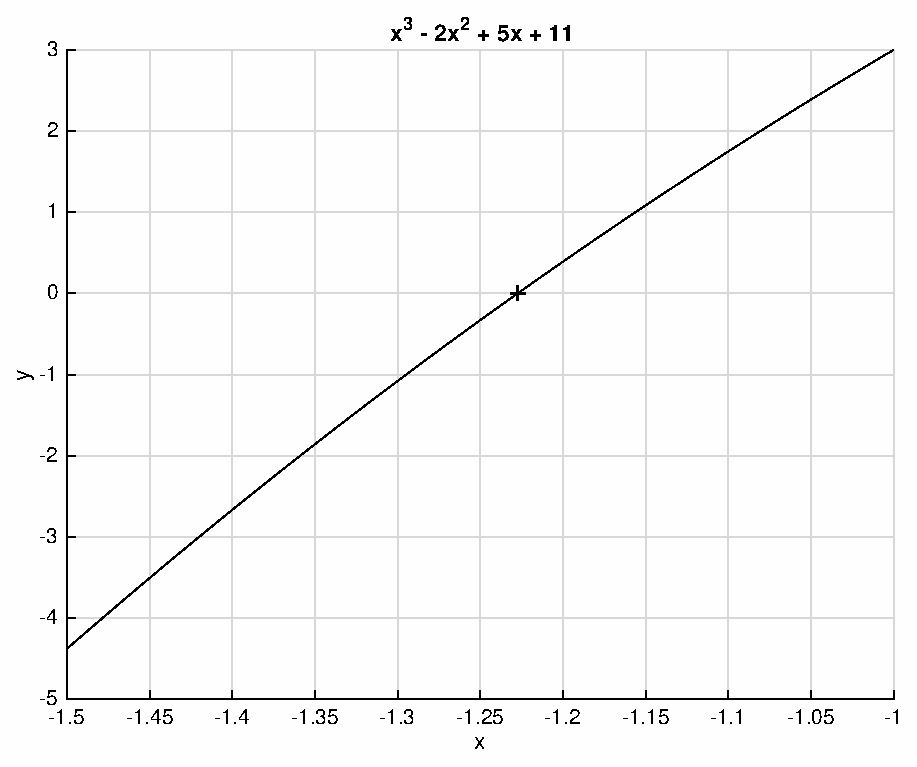
\includegraphics{graph}
\end{figure} 
\pagebreak
\paragraph{Wilkinson's polynomial}\mbox{}\\

Wilkinson's polynomials are a family of polynmials with deceptively sensitive roots. The Wilkinson polynomial of degree $n$ has as roots the integers from $1$ to $n$

\begin{figure}
    \centering
    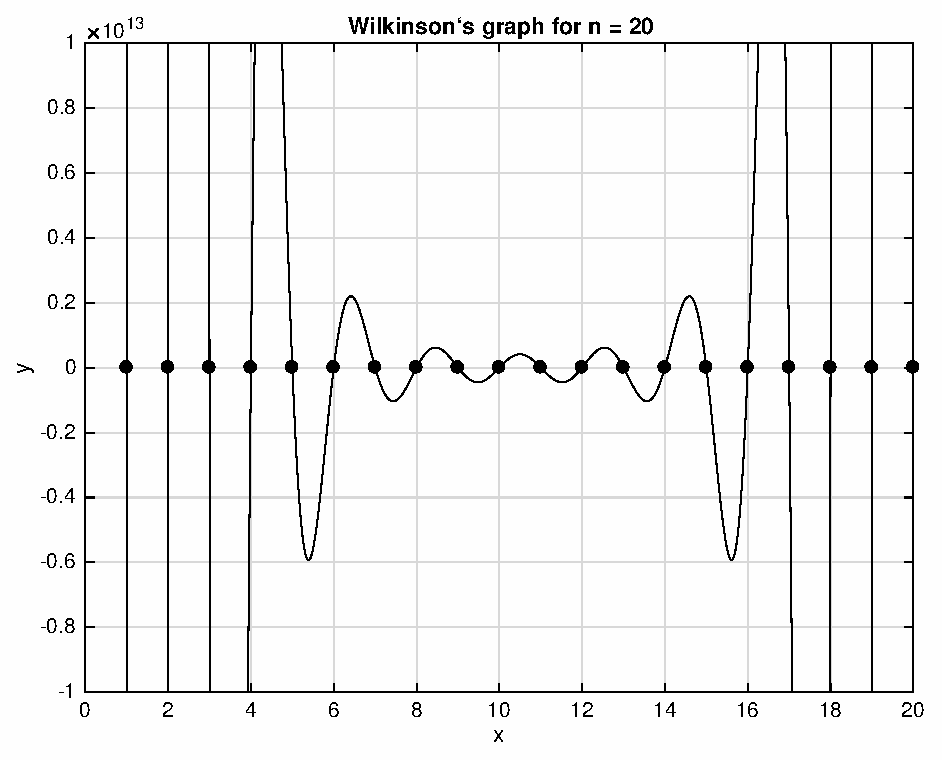
\includegraphics{wilkinsons-graph}
\end{figure} 	

\begin{figure}
    \centering
    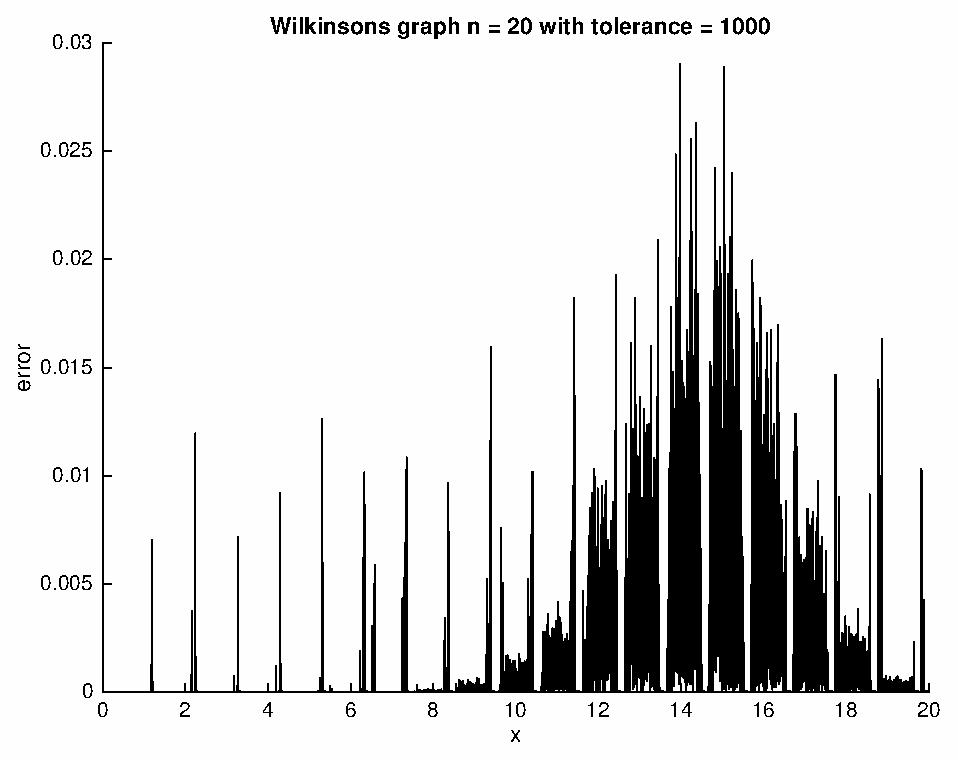
\includegraphics{test-wilkinsons-tol10-max1000.eps}
\end{figure} 	

\begin{figure}
    \centering
    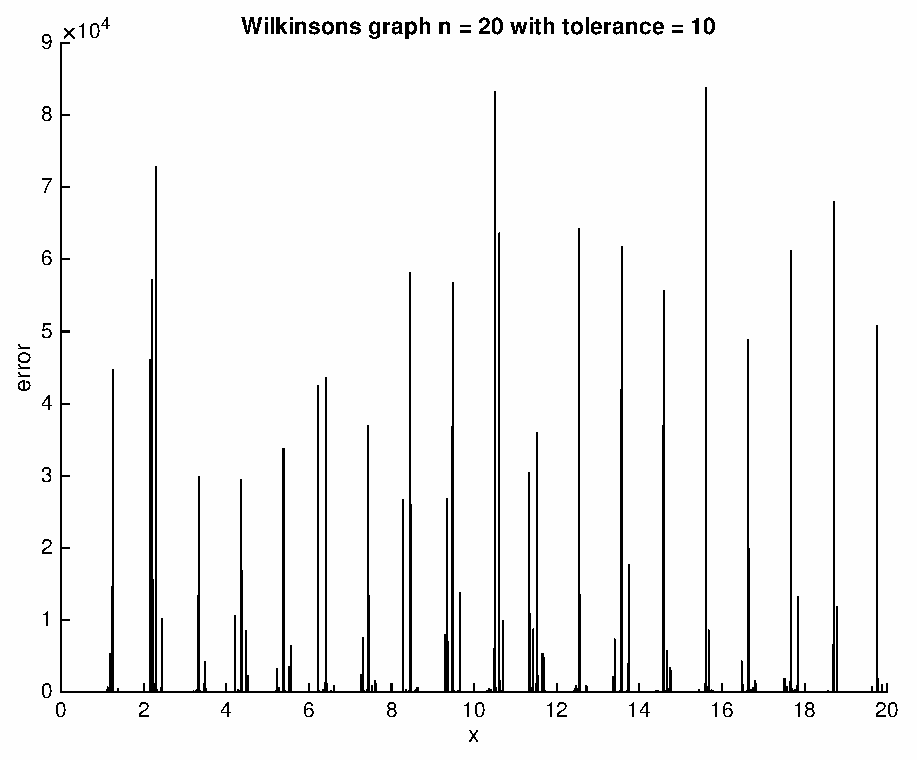
\includegraphics{test-wilkinsons-tol10-max100.eps}
\end{figure}

\[
P_{n}(x) = \prod_{k=1}^{n}(x-k).
\]

\end{document}
